\documentclass[12pt,letterpaper]{article}\usepackage[]{graphicx}\usepackage[]{color}
%% maxwidth is the original width if it is less than linewidth
%% otherwise use linewidth (to make sure the graphics do not exceed the margin)
\makeatletter
\def\maxwidth{ %
  \ifdim\Gin@nat@width>\linewidth
    \linewidth
  \else
    \Gin@nat@width
  \fi
}
\makeatother

\definecolor{fgcolor}{rgb}{0.345, 0.345, 0.345}
\newcommand{\hlnum}[1]{\textcolor[rgb]{0.686,0.059,0.569}{#1}}%
\newcommand{\hlstr}[1]{\textcolor[rgb]{0.192,0.494,0.8}{#1}}%
\newcommand{\hlcom}[1]{\textcolor[rgb]{0.678,0.584,0.686}{\textit{#1}}}%
\newcommand{\hlopt}[1]{\textcolor[rgb]{0,0,0}{#1}}%
\newcommand{\hlstd}[1]{\textcolor[rgb]{0.345,0.345,0.345}{#1}}%
\newcommand{\hlkwa}[1]{\textcolor[rgb]{0.161,0.373,0.58}{\textbf{#1}}}%
\newcommand{\hlkwb}[1]{\textcolor[rgb]{0.69,0.353,0.396}{#1}}%
\newcommand{\hlkwc}[1]{\textcolor[rgb]{0.333,0.667,0.333}{#1}}%
\newcommand{\hlkwd}[1]{\textcolor[rgb]{0.737,0.353,0.396}{\textbf{#1}}}%

\usepackage{framed}
\makeatletter
\newenvironment{kframe}{%
 \def\at@end@of@kframe{}%
 \ifinner\ifhmode%
  \def\at@end@of@kframe{\end{minipage}}%
  \begin{minipage}{\columnwidth}%
 \fi\fi%
 \def\FrameCommand##1{\hskip\@totalleftmargin \hskip-\fboxsep
 \colorbox{shadecolor}{##1}\hskip-\fboxsep
     % There is no \\@totalrightmargin, so:
     \hskip-\linewidth \hskip-\@totalleftmargin \hskip\columnwidth}%
 \MakeFramed {\advance\hsize-\width
   \@totalleftmargin\z@ \linewidth\hsize
   \@setminipage}}%
 {\par\unskip\endMakeFramed%
 \at@end@of@kframe}
\makeatother

\definecolor{shadecolor}{rgb}{.97, .97, .97}
\definecolor{messagecolor}{rgb}{0, 0, 0}
\definecolor{warningcolor}{rgb}{1, 0, 1}
\definecolor{errorcolor}{rgb}{1, 0, 0}
\newenvironment{knitrout}{}{} % an empty environment to be redefined in TeX

\usepackage{alltt}
\usepackage[left=2cm,right=2cm,top=2cm,bottom=2cm]{geometry}
\usepackage[ansinew]{inputenc}
\usepackage[spanish]{babel}
\usepackage{amsmath}
\usepackage{amsfonts}
\usepackage{amssymb}
\usepackage{dsfont}
\usepackage{multicol} 
\usepackage{subfigure}
\usepackage{graphicx}
\usepackage{float} 
\usepackage{verbatim} 
\usepackage[left=2cm,right=2cm,top=2cm,bottom=2cm]{geometry}
\usepackage{fancyhdr}
\pagestyle{fancy} 
\fancyhead[LO]{\leftmark}
\usepackage{caption}
\newtheorem{definicion}{Definci\'on}
\IfFileExists{upquote.sty}{\usepackage{upquote}}{}
\begin{document}

\begin{titlepage}
\setlength{\unitlength}{1 cm} %Especificar unidad de trabajo

\begin{center}
\textbf{{\large UNIVERSIDAD DE EL SALVADOR}\\
{\large FACULTAD MULTIDISCIPLINARIA DE OCCIDENTE}\\
{\large DEPARTAMENTO DE MATEM\'ATICA}}\\ [0.50 cm]

\begin{picture}(18,4)
 \put(7,0){
\includegraphics[width=4cm]{minerva.jpg}}
\end{picture}
\\[0.25 cm]

\textbf{{\large Licenciatura en Estad\'istica}\\ [1.25cm]
{\large Control Estad\'istico del Paquete R }\\ [2 cm]
%\setlength{\unitlength}{1 cm}
{\large  \textbf{''UNIDAD DOS"}}\\ [3 cm]
{\large Alumna:}\\
{\large Erika Beatr\'iz Guill\'en Pineda}\\ [2cm]
{\large Fecha de elaboraci\'on}\\
Santa Ana - \today }
\end{center}
\end{titlepage}

\newtheorem{teorema}{Teorema}
\newtheorem{prop}{Proposici\'on}[section]

\lhead{Pr\'actica 08}

\lfoot{LICENCIATURA EN ESTAD\'ISTICA}
\cfoot{UESOCC}
\rfoot{\thepage}
%\pagestyle{fancy} 

\setcounter{page}{1}
\newpage

\section {AN\'ALISIS ESTAD?STICO DE DATOS UNIVARIADOS CONTINUOS EN R}
\textbf{Ejemplo:} Para estudiar el examen de ingreso a la UES, se selecciona aleatoriamente una muestra de 60 alumnos, las notas de estos alumnos son las siguientes: (4.47, 4.47, 3.48, 5.0, 3.42, 3.78, 3.1, 3.57,
4.2, 4.5, 3.6, 3.75, 4.5, 2.85, 3.7, 4.2, 3.2, 4.05, 4.9, 5.1, 5.3, 4.16, 4.56, 3.54, 3.5, 5.2, 4.71, 
3.7, 4.78, 4.14, 4.14, 4.8, 4.1, 3.83, 3.6, 2.98, 4.32, 5.1, 4.3, 3.9, 3.96, 3.54, 4.8, 4.3, 3.39, 4.47,
3.19, 3.75, 3.1, 4.7, 3.69, 3.3, 2.85, 5.25, 4.68, 4.04, 4.44, 5.43, 3.04, 2.95)

\subsection{AN\'ALISIS ESTAD\'ISTICO DE LOS DATOS}

\textbf{1) Visualiza el directorio por defecto y activa su directorio de trabajo}
\begin{knitrout}
\definecolor{shadecolor}{rgb}{0.969, 0.969, 0.969}\color{fgcolor}\begin{kframe}
\begin{alltt}
\hlkwd{getwd}\hlstd{()}
\end{alltt}
\begin{verbatim}
## [1] "C:/Users/User/Documents/TODAS_PRACTICAS"
\end{verbatim}
\begin{alltt}
\hlkwd{setwd}\hlstd{(}\hlstr{"C:/Users/User/Documents/TODAS_PRACTICAS"}\hlstd{)}
\end{alltt}
\end{kframe}
\end{knitrout}
\textbf{2) Crea un nuevo Script y llamarle "Script08-DatosContinuos"}

\textbf{3) Crea el vector que contendr\'a los datos.}
\begin{knitrout}
\definecolor{shadecolor}{rgb}{0.969, 0.969, 0.969}\color{fgcolor}\begin{kframe}
\begin{alltt}
\hlstd{Notas} \hlkwb{<-} \hlkwd{c}\hlstd{(}\hlnum{4.47}\hlstd{,} \hlnum{4.47}\hlstd{,}\hlnum{3.48}\hlstd{,} \hlnum{5.0}\hlstd{,} \hlnum{3.42}\hlstd{,} \hlnum{3.78}\hlstd{,} \hlnum{3.1}\hlstd{,} \hlnum{3.57}\hlstd{,}
\hlnum{4.2}\hlstd{,} \hlnum{4.5}\hlstd{,} \hlnum{3.6}\hlstd{,} \hlnum{3.75}\hlstd{,} \hlnum{4.5}\hlstd{,} \hlnum{2.85}\hlstd{,} \hlnum{3.7}\hlstd{,} \hlnum{4.2}\hlstd{,} \hlnum{3.2}\hlstd{,} \hlnum{4.05}\hlstd{,} \hlnum{4.9}\hlstd{,}
\hlnum{5.1}\hlstd{,} \hlnum{5.3}\hlstd{,} \hlnum{4.16}\hlstd{,} \hlnum{4.56}\hlstd{,} \hlnum{3.54}\hlstd{,} \hlnum{3.5}\hlstd{,} \hlnum{5.2}\hlstd{,} \hlnum{4.71}\hlstd{,} \hlnum{3.7}\hlstd{,} \hlnum{4.78}\hlstd{,}
\hlnum{4.14}\hlstd{,} \hlnum{4.14}\hlstd{,} \hlnum{4.8}\hlstd{,} \hlnum{4.1}\hlstd{,} \hlnum{3.83}\hlstd{,} \hlnum{3.6}\hlstd{,} \hlnum{2.98}\hlstd{,} \hlnum{4.32}\hlstd{,} \hlnum{5.1}\hlstd{,} \hlnum{4.3}\hlstd{,}
\hlnum{3.9}\hlstd{,} \hlnum{3.96}\hlstd{,} \hlnum{3.54}\hlstd{,} \hlnum{4.8}\hlstd{,} \hlnum{4.3}\hlstd{,} \hlnum{3.39}\hlstd{,} \hlnum{4.47}\hlstd{,}\hlnum{3.19}\hlstd{,} \hlnum{3.75}\hlstd{,} \hlnum{3.1}\hlstd{,}
\hlnum{4.7}\hlstd{,} \hlnum{3.69}\hlstd{,} \hlnum{3.3}\hlstd{,} \hlnum{2.85}\hlstd{,} \hlnum{5.25}\hlstd{,} \hlnum{4.68}\hlstd{,} \hlnum{4.04}\hlstd{,} \hlnum{4.44}\hlstd{,} \hlnum{5.43}\hlstd{,} \hlnum{3.04}\hlstd{,} \hlnum{2.95}\hlstd{);}
\hlstd{Notas}
\end{alltt}
\begin{verbatim}
##  [1] 4.47 4.47 3.48 5.00 3.42 3.78 3.10 3.57 4.20 4.50 3.60 3.75 4.50 2.85
## [15] 3.70 4.20 3.20 4.05 4.90 5.10 5.30 4.16 4.56 3.54 3.50 5.20 4.71 3.70
## [29] 4.78 4.14 4.14 4.80 4.10 3.83 3.60 2.98 4.32 5.10 4.30 3.90 3.96 3.54
## [43] 4.80 4.30 3.39 4.47 3.19 3.75 3.10 4.70 3.69 3.30 2.85 5.25 4.68 4.04
## [57] 4.44 5.43 3.04 2.95
\end{verbatim}
\begin{alltt}
\hlkwd{data.entry}\hlstd{(Notas)}
\hlstd{Notas}
\end{alltt}
\begin{verbatim}
##  [1] 4.47 4.47 3.48 5.00 3.42 3.78 3.10 3.57 4.20 4.50 3.60 3.75 4.50 2.85
## [15] 3.70 4.20 3.20 4.05 4.90 5.10 5.30 4.16 4.56 3.54 3.50 5.20 4.71 3.70
## [29] 4.78 4.14 4.14 4.80 4.10 3.83 3.60 2.98 4.32 5.10 4.30 3.90 3.96 3.54
## [43] 4.80 4.30 3.39 4.47 3.19 3.75 3.10 4.70 3.69 3.30 2.85 5.25 4.68 4.04
## [57] 4.44 5.43 3.04 2.95
\end{verbatim}
\begin{alltt}
\hlkwd{length}\hlstd{(Notas)}
\end{alltt}
\begin{verbatim}
## [1] 60
\end{verbatim}
\end{kframe}
\end{knitrout}
\tetxbf{4) Guarda el vector de datos en un archivo.}
\begin{knitrout}
\definecolor{shadecolor}{rgb}{0.969, 0.969, 0.969}\color{fgcolor}\begin{kframe}
\begin{alltt}
\hlkwd{write}\hlstd{(Notas,} \hlstr{"Notas.txt"}\hlstd{)}
\end{alltt}
\end{kframe}
\end{knitrout}
\textbf{5) Limpia el \'area de trabajo (Workspace)}
\begin{knitrout}
\definecolor{shadecolor}{rgb}{0.969, 0.969, 0.969}\color{fgcolor}\begin{kframe}
\begin{alltt}
\hlkwd{ls}\hlstd{()}
\end{alltt}
\begin{verbatim}
## [1] "Notas"
\end{verbatim}
\begin{alltt}
\hlkwd{rm}\hlstd{(}\hlkwc{list}\hlstd{=}\hlkwd{ls}\hlstd{(}\hlkwc{all}\hlstd{=}\hlnum{TRUE}\hlstd{))}
\hlkwd{ls}\hlstd{()}
\end{alltt}
\begin{verbatim}
## character(0)
\end{verbatim}
\end{kframe}
\end{knitrout}
\textbf{6) Lee o recupera el vector de datos desde el archivo de texto}
\begin{knitrout}
\definecolor{shadecolor}{rgb}{0.969, 0.969, 0.969}\color{fgcolor}\begin{kframe}
\begin{alltt}
\hlstd{X} \hlkwb{<-} \hlkwd{scan}\hlstd{(}\hlstr{"Notas.txt"}\hlstd{,} \hlkwc{what} \hlstd{=} \hlkwd{double}\hlstd{(}\hlnum{0}\hlstd{),} \hlkwc{na.strings} \hlstd{=} \hlstr{"NA"}\hlstd{,} \hlkwc{flush}\hlstd{=}\hlnum{FALSE}\hlstd{)}
\hlkwd{ls}\hlstd{()}
\end{alltt}
\begin{verbatim}
## [1] "X"
\end{verbatim}
\begin{alltt}
\hlcom{# Si el vector contiene valores reales se ocupa: what = double(0)}
\end{alltt}
\end{kframe}
\end{knitrout}
\textbf{7) Crea la tabla de frecuencias}
\begin{knitrout}
\definecolor{shadecolor}{rgb}{0.969, 0.969, 0.969}\color{fgcolor}\begin{kframe}
\begin{alltt}
\hlcom{# Define el nvumero k de los intervalos o clases.}
\hlcom{# Usa el M\textbackslash{}'etodo de Herbert A. Sturges para determinar dicho n?mero.}
\hlstd{n} \hlkwb{<-} \hlkwd{length}\hlstd{(X); n}
\end{alltt}
\begin{verbatim}
## [1] 60
\end{verbatim}
\begin{alltt}
\hlstd{k} \hlkwb{<-} \hlnum{1}\hlopt{+}\hlnum{3.322}\hlopt{*}\hlkwd{logb}\hlstd{(n,} \hlnum{10}\hlstd{); k}
\end{alltt}
\begin{verbatim}
## [1] 6.907018
\end{verbatim}
\begin{alltt}
\hlstd{k} \hlkwb{<-} \hlkwd{round}\hlstd{(k); k}
\end{alltt}
\begin{verbatim}
## [1] 7
\end{verbatim}
\begin{alltt}
\hlcom{# Calcula el ancho o amplitud a de cada intervalo a=rango/k}
\hlstd{rango} \hlkwb{<-} \hlkwd{max}\hlstd{(X)}\hlopt{-}\hlkwd{min}\hlstd{(X);}
\hlstd{rango}
\end{alltt}
\begin{verbatim}
## [1] 2.58
\end{verbatim}
\begin{alltt}
\hlstd{a}\hlkwb{=}\hlstd{rango}\hlopt{/}\hlstd{k;}
\hlstd{a}
\end{alltt}
\begin{verbatim}
## [1] 0.3685714
\end{verbatim}
\begin{alltt}
\hlstd{a} \hlkwb{<-} \hlkwd{round}\hlstd{(a,} \hlnum{3}\hlstd{);}
\hlstd{a}
\end{alltt}
\begin{verbatim}
## [1] 0.369
\end{verbatim}
\begin{alltt}
\hlcom{# Define los l\textbackslash{}'imites y puntos medios de cada uno de los k intervalos}
\hlstd{limites} \hlkwb{<-} \hlkwd{seq}\hlstd{(}\hlkwc{from}\hlstd{=}\hlkwd{min}\hlstd{(X)}\hlopt{-}\hlnum{0.01}\hlopt{/}\hlnum{2}\hlstd{,} \hlkwc{to}\hlstd{=}\hlkwd{max}\hlstd{(X)}\hlopt{+}\hlnum{0.01}\hlopt{/}\hlnum{2}\hlstd{,} \hlkwc{by}\hlstd{=a);}
\hlstd{limites}
\end{alltt}
\begin{verbatim}
## [1] 2.845 3.214 3.583 3.952 4.321 4.690 5.059 5.428
\end{verbatim}
\begin{alltt}
\hlkwd{options}\hlstd{(}\hlkwc{digits}\hlstd{=}\hlnum{4}\hlstd{)}
\hlstd{ci} \hlkwb{<-} \hlkwd{cbind}\hlstd{(}\hlnum{1}\hlopt{:}\hlstd{k);}
\hlstd{ci}
\end{alltt}
\begin{verbatim}
##      [,1]
## [1,]    1
## [2,]    2
## [3,]    3
## [4,]    4
## [5,]    5
## [6,]    6
## [7,]    7
\end{verbatim}
\begin{alltt}
\hlkwa{for}\hlstd{(i} \hlkwa{in} \hlnum{2}\hlopt{:}\hlkwd{length}\hlstd{(limites)) ci[i}\hlopt{-}\hlnum{1}\hlstd{,} \hlnum{1}\hlstd{]} \hlkwb{<-} \hlstd{(limites[i]} \hlopt{+} \hlstd{limites[i}\hlopt{-}\hlnum{1}\hlstd{])}\hlopt{/}\hlnum{2}
\hlstd{ci}
\end{alltt}
\begin{verbatim}
##       [,1]
## [1,] 3.030
## [2,] 3.399
## [3,] 3.768
## [4,] 4.136
## [5,] 4.505
## [6,] 4.875
## [7,] 5.244
\end{verbatim}
\begin{alltt}
\hlcom{# Encuentra las frecuencias absolutas fi para cada intervalo.}
\hlkwd{options}\hlstd{(}\hlkwc{digits}\hlstd{=}\hlnum{2}\hlstd{)}
\hlstd{fi} \hlkwb{<-} \hlkwd{cbind}\hlstd{(}\hlkwd{table}\hlstd{(}\hlkwd{cut}\hlstd{(X,} \hlkwc{breaks} \hlstd{= limites,} \hlkwc{labels}\hlstd{=}\hlkwa{NULL}\hlstd{,} \hlkwc{include.lowest}\hlstd{=}\hlnum{FALSE}\hlstd{,}
\hlkwc{right}\hlstd{=}\hlnum{FALSE}\hlstd{,} \hlkwc{dig.lab}\hlstd{=}\hlnum{4}\hlstd{)));}
\hlstd{fi}
\end{alltt}
\begin{verbatim}
##               [,1]
## [2.845,3.214)    9
## [3.214,3.583)    8
## [3.583,3.952)   10
## [3.952,4.321)   12
## [4.321,4.69)     8
## [4.69,5.059)     7
## [5.059,5.428)    5
\end{verbatim}
\begin{alltt}
\hlcom{# breaks es un vector o secuencia de cortes 1:6, o el n\textbackslash{}'umero de clases.}
\hlcom{# labels indica que no hay nombres para los intervalos o clases, por }
\hlcom{# defecto las etiquetas tienen la notaci\textbackslash{}'on (a, b]}
\hlcom{# include.lowest indica que si un X[i] es igual al corte inferior }
\hlcom{# (0 superior, para right=FALSE) el valor debe ser incluido.}
\hlcom{# right indica que s\textbackslash{}'i el intervalo debe ser cerrado a la derecha }
\hlcom{# y abierto a la izquierda, o viceversa.}
\hlcom{# dig.lab es un entero el cual es usado cuando las etiquetas no }
\hlcom{# son dadas, determina el n\textbackslash{}'umero de d\textbackslash{}'igitos usado en el formato de }
\hlcom{# n\textbackslash{}'umeros de cortes.Encuentra las frecuencias relativas o proporciones fri.}
\hlcom{# options(digits=4)}
\hlstd{fri} \hlkwb{<-} \hlstd{fi}\hlopt{/}\hlstd{n;}
\hlstd{fri}
\end{alltt}
\begin{verbatim}
##                [,1]
## [2.845,3.214) 0.150
## [3.214,3.583) 0.133
## [3.583,3.952) 0.167
## [3.952,4.321) 0.200
## [4.321,4.69)  0.133
## [4.69,5.059)  0.117
## [5.059,5.428) 0.083
\end{verbatim}
\begin{alltt}
\hlcom{# Encuentra las frecuencias acumuladas ascendentes Fi}
\hlkwd{options}\hlstd{(}\hlkwc{digits}\hlstd{=}\hlnum{2}\hlstd{)}
\hlstd{Fi} \hlkwb{<-} \hlkwd{cumsum}\hlstd{(fi);}
\hlstd{Fi}
\end{alltt}
\begin{verbatim}
## [1]  9 17 27 39 47 54 59
\end{verbatim}
\begin{alltt}
\hlcom{# Encuentra las frecuencias relativas acumuladas Fri}
\hlkwd{options}\hlstd{(}\hlkwc{digits}\hlstd{=}\hlnum{4}\hlstd{)}
\hlstd{Fri} \hlkwb{<-} \hlstd{Fi}\hlopt{/}\hlstd{n;}
\hlstd{Fri}
\end{alltt}
\begin{verbatim}
## [1] 0.1500 0.2833 0.4500 0.6500 0.7833 0.9000 0.9833
\end{verbatim}
\begin{alltt}
\hlcom{# Completa la tabla de frecuencias.}
\hlstd{tablaFrec} \hlkwb{<-} \hlkwd{data.frame}\hlstd{(}\hlkwc{ci}\hlstd{=ci,} \hlkwc{fi}\hlstd{=fi,} \hlkwc{fri}\hlstd{=fri,} \hlkwc{Fi}\hlstd{=Fi,} \hlkwc{Fri}\hlstd{=Fri);}
\hlstd{tablaFrec}
\end{alltt}
\begin{verbatim}
##                  ci fi     fri Fi    Fri
## [2.845,3.214) 3.030  9 0.15000  9 0.1500
## [3.214,3.583) 3.399  8 0.13333 17 0.2833
## [3.583,3.952) 3.768 10 0.16667 27 0.4500
## [3.952,4.321) 4.136 12 0.20000 39 0.6500
## [4.321,4.69)  4.505  8 0.13333 47 0.7833
## [4.69,5.059)  4.875  7 0.11667 54 0.9000
## [5.059,5.428) 5.244  5 0.08333 59 0.9833
\end{verbatim}
\begin{alltt}
\hlcom{# Nuevamente puede usar el comando xtable para importar a c?digo LATEX.}
\end{alltt}
\end{kframe}
\end{knitrout}
\textbf{8?) Crea el histograma de frecuencias}
\begin{knitrout}
\definecolor{shadecolor}{rgb}{0.969, 0.969, 0.969}\color{fgcolor}\begin{kframe}
\begin{alltt}
\hlstd{h} \hlkwb{<-} \hlkwd{hist}\hlstd{(X,} \hlkwc{breaks}\hlstd{=}\hlkwd{c}\hlstd{(limites[}\hlnum{1}\hlstd{]}\hlopt{-}\hlstd{a, limites, limites[k}\hlopt{+}\hlnum{1}\hlstd{]}\hlopt{+}\hlstd{a),} \hlkwc{freq} \hlstd{=} \hlnum{TRUE}\hlstd{,}
          \hlkwc{probability} \hlstd{=} \hlnum{FALSE}\hlstd{,} \hlkwc{include.lowest} \hlstd{=} \hlnum{FALSE}\hlstd{,}\hlkwc{right} \hlstd{=} \hlnum{TRUE}\hlstd{,}
          \hlkwc{main} \hlstd{=} \hlstr{"Histograma de frecuencias"}\hlstd{,} \hlkwc{col}\hlstd{=}\hlstr{"lightyellow"}\hlstd{,} \hlkwc{lty}\hlstd{=}\hlnum{1}\hlstd{,}
          \hlkwc{border}\hlstd{=}\hlstr{"purple"}\hlstd{,} \hlkwc{xlab}\hlstd{=}\hlstr{" Notas de aspirantes"}\hlstd{,} \hlkwc{ylab}\hlstd{=}\hlstr{"Frecuencia (fi)"}\hlstd{,}
\hlkwc{axes}\hlstd{=}\hlnum{TRUE}\hlstd{,} \hlkwc{labels}\hlstd{=}\hlnum{FALSE}\hlstd{)}
\hlkwd{text}\hlstd{(h}\hlopt{$}\hlstd{mids, h}\hlopt{$}\hlstd{density, h}\hlopt{$}\hlstd{counts,} \hlkwc{adj}\hlstd{=}\hlkwd{c}\hlstd{(}\hlnum{0.5}\hlstd{,} \hlopt{-}\hlnum{0.5}\hlstd{),} \hlkwc{col}\hlstd{=}\hlstr{"red"}\hlstd{)}
\hlkwd{rug}\hlstd{(}\hlkwd{jitter}\hlstd{(X))} \hlcom{# Adiciona marcas de los datos}
\end{alltt}
\end{kframe}
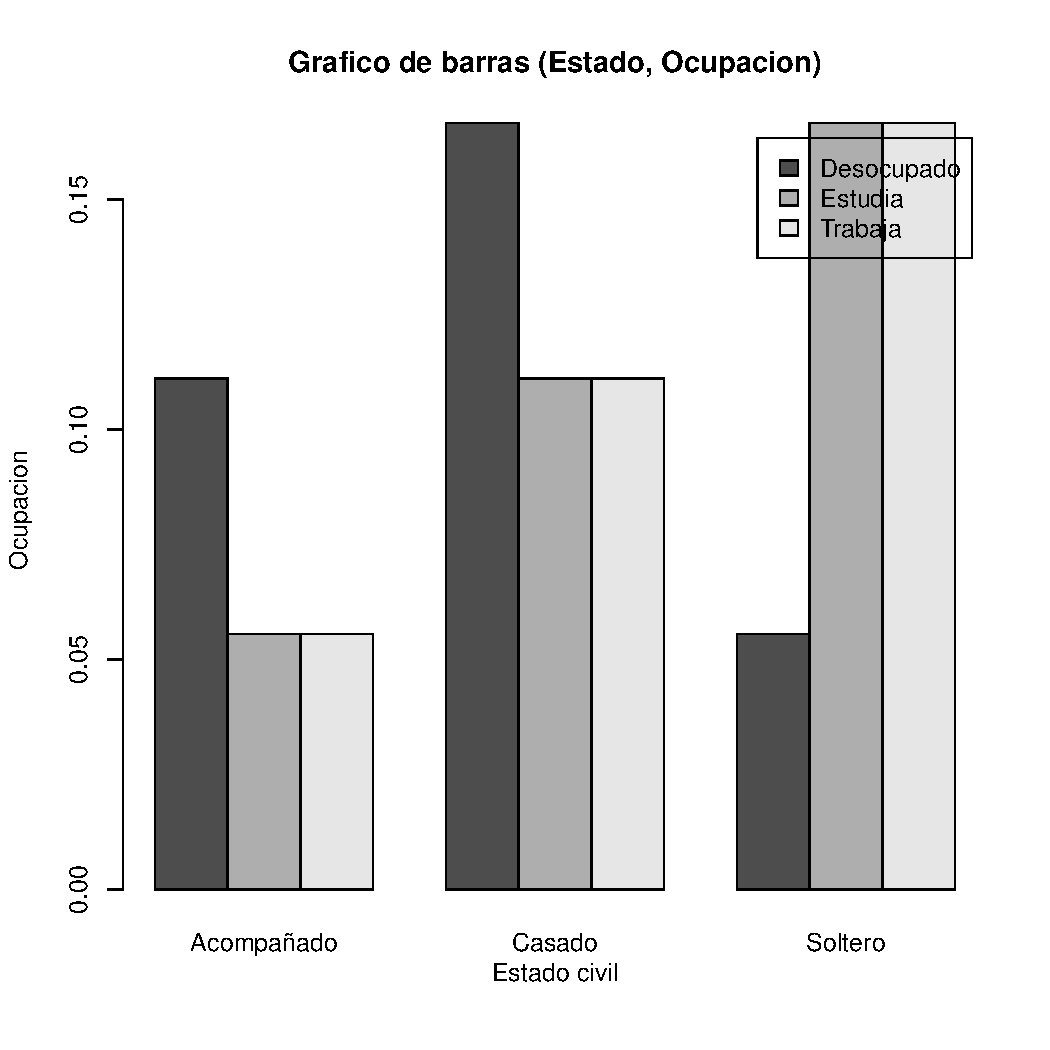
\includegraphics[width=\maxwidth]{figure/unnamed-chunk-7-1} 
\begin{kframe}\begin{alltt}
\hlcom{# h es un objeto del tipo lista que contiene atributos del histograma}
\hlkwd{is.list}\hlstd{(h);}
\end{alltt}
\begin{verbatim}
## [1] TRUE
\end{verbatim}
\begin{alltt}
\hlstd{h}
\end{alltt}
\begin{verbatim}
## $breaks
##  [1] 2.476 2.845 3.214 3.583 3.952 4.321 4.690 5.059 5.428 5.797
## 
## $counts
## [1]  0  9  8 10 12  8  7  5  1
## 
## $density
## [1] 0.00000 0.40650 0.36134 0.45167 0.54201 0.36134 0.31617 0.22584 0.04517
## 
## $mids
## [1] 2.660 3.030 3.399 3.768 4.136 4.505 4.875 5.244 5.613
## 
## $xname
## [1] "X"
## 
## $equidist
## [1] TRUE
## 
## attr(,"class")
## [1] "histogram"
\end{verbatim}
\end{kframe}
\end{knitrout}
\textbf{9) Aproxima al histograma la funci\'on de densidad normal}
\begin{knitrout}
\definecolor{shadecolor}{rgb}{0.969, 0.969, 0.969}\color{fgcolor}\begin{kframe}
\begin{alltt}
\hlstd{h} \hlkwb{<-} \hlkwd{hist}\hlstd{(X,} \hlkwc{breaks}\hlstd{=}\hlkwd{c}\hlstd{(limites[}\hlnum{1}\hlstd{]}\hlopt{-}\hlstd{a, limites, limites[k}\hlopt{+}\hlnum{1}\hlstd{]}\hlopt{+}\hlstd{a),} \hlkwc{freq} \hlstd{=} \hlnum{FALSE}\hlstd{,}
\hlkwc{probability} \hlstd{=} \hlnum{TRUE}\hlstd{,} \hlkwc{include.lowest} \hlstd{=} \hlnum{FALSE}\hlstd{,} \hlkwc{right} \hlstd{=} \hlnum{TRUE}\hlstd{,}
\hlkwc{main}\hlstd{=}\hlstr{"Aproximacion a una Normal\textbackslash{}n"}\hlstd{,} \hlkwc{col}\hlstd{=}\hlstr{"lightyellow"}\hlstd{,}\hlkwc{lty}\hlstd{=}\hlnum{1}\hlstd{,}\hlkwc{border}\hlstd{=}\hlstr{"purple"}\hlstd{,}
\hlkwc{xlab}\hlstd{=}\hlstr{"Notas de aspirantes\textbackslash{}n"}\hlstd{,} \hlkwc{ylab}\hlstd{=}\hlstr{"Frecuencia relativa (fri)"}\hlstd{,}
\hlkwc{axes}\hlstd{=}\hlnum{TRUE}\hlstd{,} \hlkwc{labels}\hlstd{=}\hlnum{FALSE}\hlstd{)}
\hlkwd{text}\hlstd{(h}\hlopt{$}\hlstd{mids, h}\hlopt{$}\hlstd{density, h}\hlopt{$}\hlstd{counts,} \hlkwc{adj}\hlstd{=}\hlkwd{c}\hlstd{(}\hlnum{0.5}\hlstd{,} \hlnum{0.2}\hlstd{),} \hlkwc{col}\hlstd{=}\hlstr{"red"}\hlstd{)}
\hlkwd{rug}\hlstd{(}\hlkwd{jitter}\hlstd{(X))} \hlcom{# Adiciona marcas de los datos}
\hlkwd{curve}\hlstd{(}\hlkwd{dnorm}\hlstd{(x,} \hlkwc{mean}\hlstd{=}\hlkwd{mean}\hlstd{(X),} \hlkwc{sd}\hlstd{=}\hlkwd{sd}\hlstd{(X)),} \hlkwc{col} \hlstd{=} \hlnum{2}\hlstd{,} \hlkwc{lty} \hlstd{=} \hlnum{2}\hlstd{,}\hlkwc{lwd} \hlstd{=} \hlnum{2}\hlstd{,} \hlkwc{add} \hlstd{=} \hlnum{TRUE}\hlstd{)}
\end{alltt}
\end{kframe}
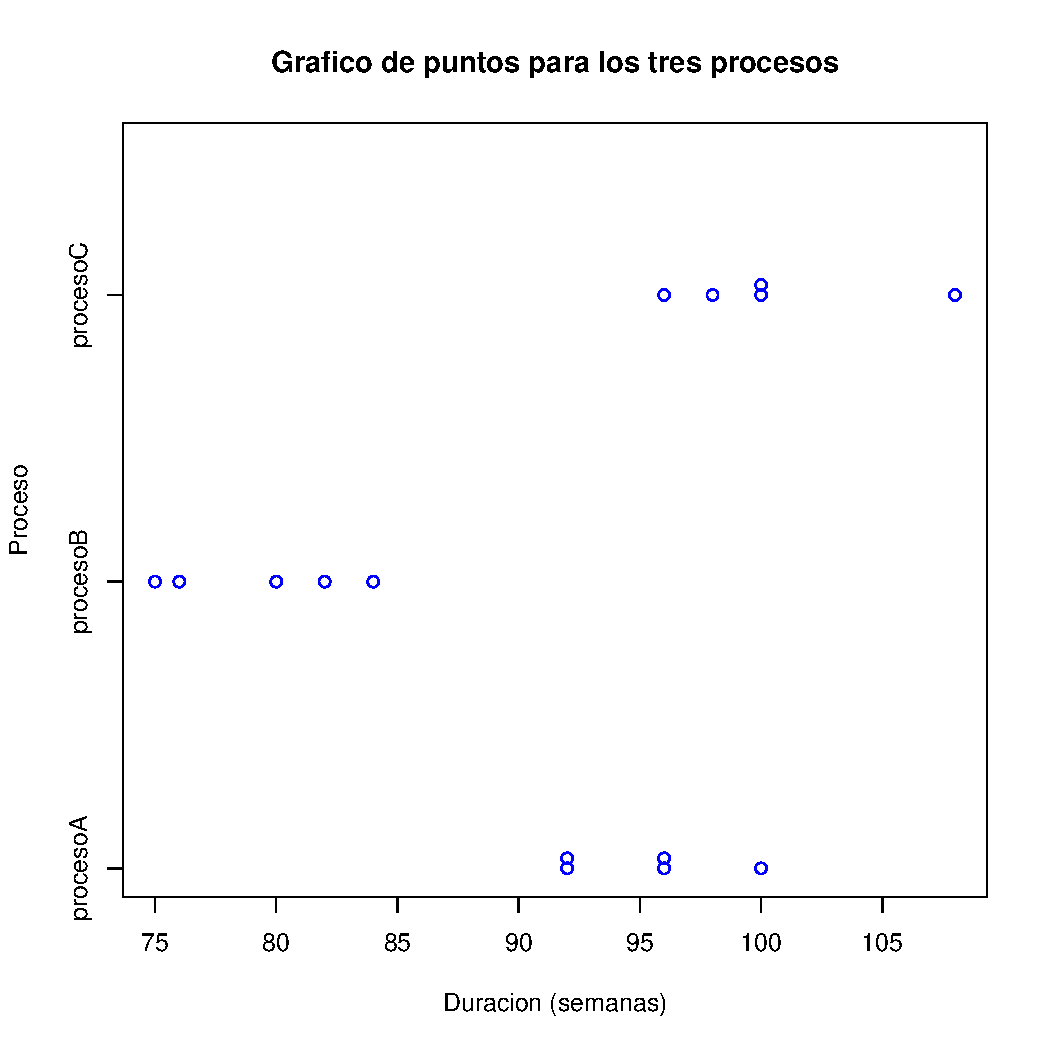
\includegraphics[width=\maxwidth]{figure/unnamed-chunk-8-1} 

\end{knitrout}
\textbf{10) Crea el pol\'igono de frecuencias}
\begin{knitrout}
\definecolor{shadecolor}{rgb}{0.969, 0.969, 0.969}\color{fgcolor}\begin{kframe}
\begin{alltt}
\hlstd{h} \hlkwb{<-} \hlkwd{hist}\hlstd{(X,} \hlkwc{breaks}\hlstd{=}\hlkwd{c}\hlstd{(limites[}\hlnum{1}\hlstd{]}\hlopt{-}\hlstd{a, limites, limites[k}\hlopt{+}\hlnum{1}\hlstd{]}\hlopt{+}\hlstd{a),} \hlkwc{freq} \hlstd{=} \hlnum{TRUE}\hlstd{,}
\hlkwc{probability}\hlstd{=}\hlnum{FALSE}\hlstd{,} \hlkwc{include.lowest}\hlstd{=}\hlnum{FALSE}\hlstd{,}\hlkwc{right}\hlstd{=}\hlnum{TRUE}\hlstd{,}
\hlkwc{main} \hlstd{=} \hlstr{"Poligono de frecuencias"}\hlstd{,}\hlkwc{col}\hlstd{=}\hlstr{"lightyellow"}\hlstd{,} \hlkwc{lty}\hlstd{=}\hlnum{1}\hlstd{,} \hlkwc{border}\hlstd{=}\hlstr{"purple"}\hlstd{,}
\hlkwc{xlab}\hlstd{=}\hlstr{"Notas de aspirantes"}\hlstd{,} \hlkwc{ylab}\hlstd{=}\hlstr{"Frecuencia (fi)"}\hlstd{,} \hlkwc{axes}\hlstd{=}\hlnum{TRUE}\hlstd{,} \hlkwc{labels}\hlstd{=}\hlnum{FALSE}\hlstd{)}
\hlkwd{text}\hlstd{(h}\hlopt{$}\hlstd{mids, h}\hlopt{$}\hlstd{density, h}\hlopt{$}\hlstd{counts,} \hlkwc{adj}\hlstd{=}\hlkwd{c}\hlstd{(}\hlnum{0.5}\hlstd{,} \hlopt{-}\hlnum{0.5}\hlstd{),} \hlkwc{col}\hlstd{=}\hlstr{"red"}\hlstd{)}
\hlkwd{rug}\hlstd{(}\hlkwd{jitter}\hlstd{(X))} \hlcom{# adiciona marcas de los datos}
\hlstd{vCi} \hlkwb{<-} \hlkwd{c}\hlstd{(h}\hlopt{$}\hlstd{mids[}\hlnum{1}\hlstd{]}\hlopt{-}\hlstd{a, h}\hlopt{$}\hlstd{mids, h}\hlopt{$}\hlstd{mids[k}\hlopt{+}\hlnum{1}\hlstd{]}\hlopt{+}\hlstd{a);}
\hlstd{vCi}
\end{alltt}
\begin{verbatim}
##  [1] 2.292 2.660 3.030 3.399 3.768 4.136 4.505 4.875 5.244 5.613 5.613
\end{verbatim}
\begin{alltt}
\hlstd{vfi} \hlkwb{<-} \hlkwd{c}\hlstd{(}\hlnum{0}\hlstd{, h}\hlopt{$}\hlstd{counts,} \hlnum{0}\hlstd{);}
\hlstd{vfi}
\end{alltt}
\begin{verbatim}
##  [1]  0  0  9  8 10 12  8  7  5  1  0
\end{verbatim}
\begin{alltt}
\hlkwd{lines}\hlstd{(vCi, vfi,} \hlkwc{col}\hlstd{=}\hlstr{"blue"}\hlstd{,} \hlkwc{type}\hlstd{=}\hlstr{"l"}\hlstd{)}
\end{alltt}
\end{kframe}
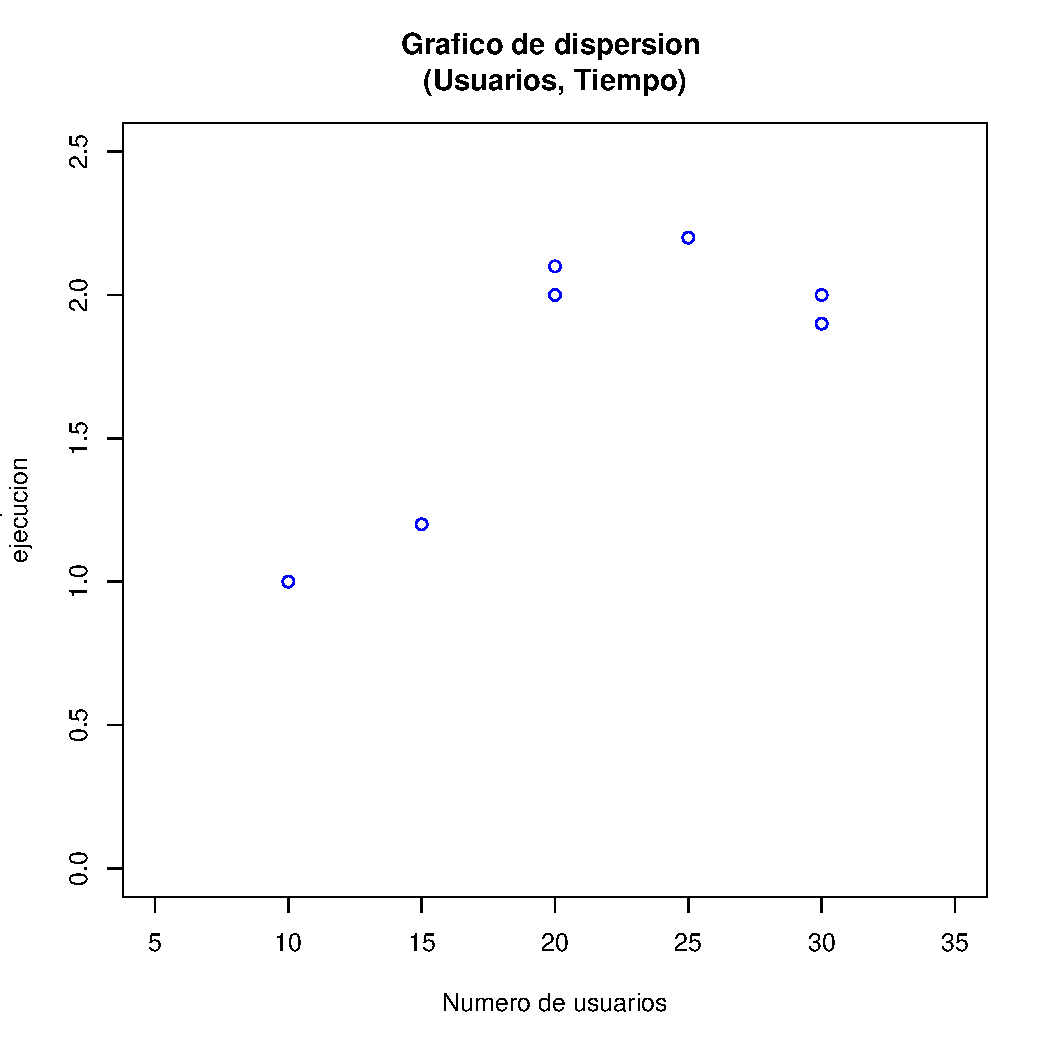
\includegraphics[width=\maxwidth]{figure/unnamed-chunk-9-1} 

\end{knitrout}
\tetxbf{11) Crea la Ojiva ascendente o pol\'igono de frecuencias acumuladas ascendentes}
\begin{knitrout}
\definecolor{shadecolor}{rgb}{0.969, 0.969, 0.969}\color{fgcolor}\begin{kframe}
\begin{alltt}
\hlstd{Fia} \hlkwb{<-} \hlkwd{c}\hlstd{(}\hlnum{0}\hlstd{, Fi); Fia}
\end{alltt}
\begin{verbatim}
## [1]  0  9 17 27 39 47 54 59
\end{verbatim}
\begin{alltt}
\hlkwd{plot}\hlstd{(limites, Fia,} \hlkwc{type} \hlstd{=} \hlstr{"p"}\hlstd{,} \hlkwc{pch}\hlstd{=}\hlnum{1}\hlstd{,} \hlkwc{col} \hlstd{=} \hlstr{"blue"}\hlstd{,} \hlkwc{main}\hlstd{=}\hlstr{"Ojiva ascendente"}\hlstd{,}
\hlkwc{xlab}\hlstd{=}\hlstr{"Notas de aspirantes"}\hlstd{,} \hlkwc{ylab}\hlstd{=}\hlstr{"Frecuencia acumulada (Fi)"}\hlstd{)}
\hlkwd{text}\hlstd{(limites, h}\hlopt{$}\hlstd{density, Fia,} \hlkwc{adj}\hlstd{=}\hlkwd{c}\hlstd{(}\hlnum{0.5}\hlstd{,} \hlopt{-}\hlnum{0.5}\hlstd{),} \hlkwc{col}\hlstd{=}\hlstr{"red"}\hlstd{)}
\hlkwd{lines}\hlstd{(limites, Fia,} \hlkwc{col}\hlstd{=}\hlstr{"black"}\hlstd{,} \hlkwc{type}\hlstd{=}\hlstr{"l"}\hlstd{)}
\end{alltt}
\end{kframe}
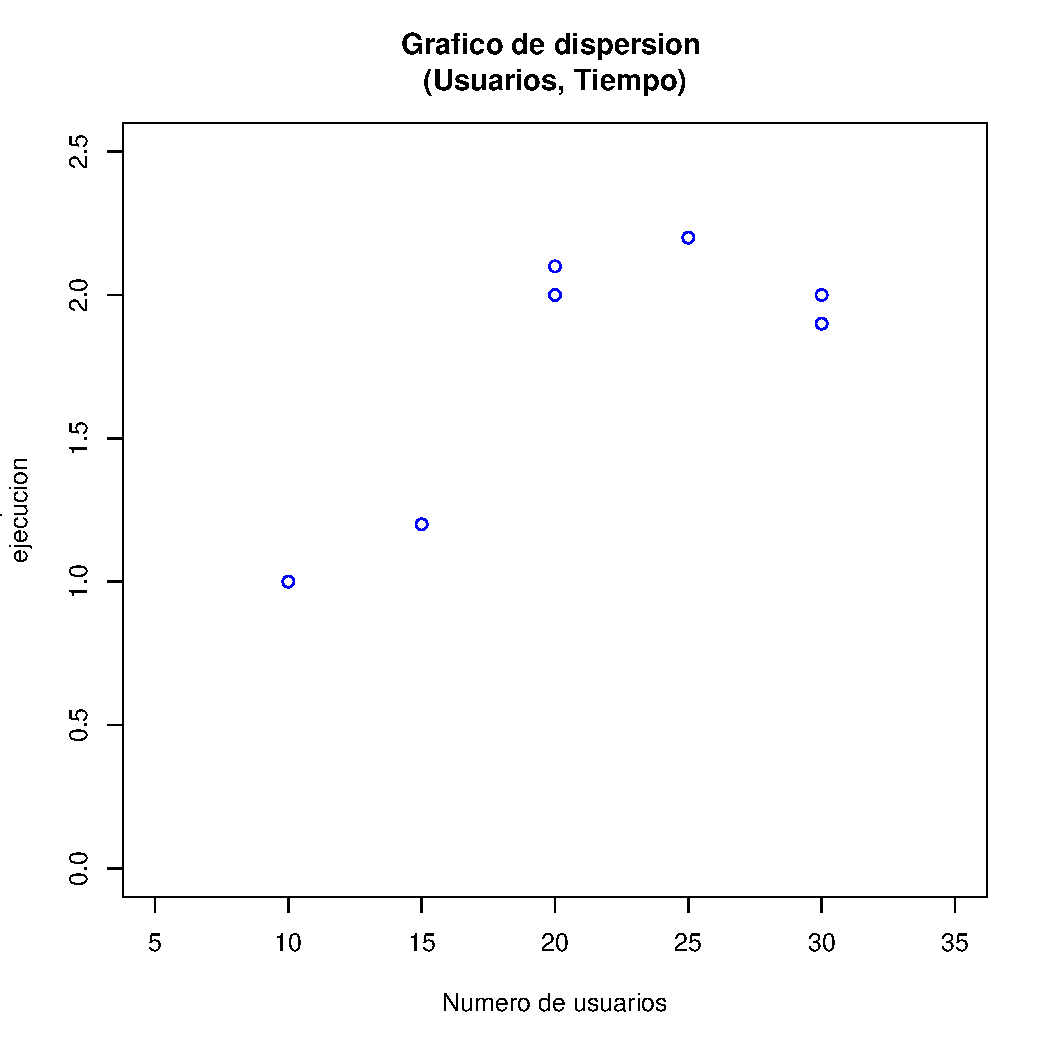
\includegraphics[width=\maxwidth]{figure/unnamed-chunk-10-1} 

\end{knitrout}
\textbf{12) Calcula los principales estad\'isticos descriptivos de la variable}
\begin{knitrout}
\definecolor{shadecolor}{rgb}{0.969, 0.969, 0.969}\color{fgcolor}\begin{kframe}
\begin{alltt}
\hlcom{# Calcula la moda, ya que el R no proporciona una funci\textbackslash{}'on para eso.}
\hlkwd{options}\hlstd{(}\hlkwc{digits}\hlstd{=}\hlnum{4}\hlstd{)}
\hlkwa{for}\hlstd{(i} \hlkwa{in} \hlnum{1}\hlopt{:}\hlstd{k)} \hlkwa{if} \hlstd{(fi[i]} \hlopt{==} \hlkwd{max}\hlstd{(fi))} \hlkwa{break}\hlstd{()}
\hlstd{\{}\hlkwa{if}\hlstd{(i} \hlopt{>} \hlnum{1}\hlstd{) moda} \hlkwb{<-} \hlstd{limites[i]}\hlopt{+}\hlstd{((fi[i]}\hlopt{-}\hlstd{fi[i}\hlopt{-}\hlnum{1}\hlstd{])}\hlopt{/}\hlstd{((fi[i]}\hlopt{-}\hlstd{fi[i}\hlopt{-}\hlnum{1}\hlstd{])}\hlopt{+}
                                          \hlstd{(fi[i]}\hlopt{-}\hlstd{fi[i}\hlopt{+}\hlnum{1}\hlstd{]) ))}\hlopt{*}\hlstd{a}
\hlkwa{else} \hlstd{moda} \hlkwb{<-} \hlstd{limites[i]}\hlopt{+}\hlstd{(fi[i]}\hlopt{/}\hlstd{(fi[i]}\hlopt{+}\hlstd{(fi[i]}\hlopt{-}\hlstd{fi[i}\hlopt{+}\hlnum{1}\hlstd{])))}\hlopt{*}\hlstd{a}
\hlstd{moda\}}
\end{alltt}
\begin{verbatim}
## [1] 4.075
\end{verbatim}
\begin{alltt}
\hlcom{# Calcula los cuartiles: Q1, Q2, Q3}
\hlstd{Q} \hlkwb{<-} \hlnum{1}\hlopt{:}\hlnum{3}
\hlkwa{for}\hlstd{(v} \hlkwa{in} \hlnum{1}\hlopt{:}\hlnum{3}\hlstd{)} \hlkwa{for}\hlstd{(i} \hlkwa{in} \hlnum{1}\hlopt{:}\hlstd{k)} \hlkwa{if} \hlstd{(Fi[i]} \hlopt{>} \hlstd{(v}\hlopt{*}\hlnum{25}\hlopt{*}\hlstd{n)}\hlopt{/}\hlnum{100}\hlstd{)}
\hlstd{\{}
\hlstd{Q[v]} \hlkwb{<-} \hlstd{limites[i]}\hlopt{+}\hlstd{(((}\hlnum{25}\hlopt{*}\hlstd{v}\hlopt{*}\hlstd{n}\hlopt{/}\hlnum{100}\hlstd{)}\hlopt{-}\hlstd{Fi[i}\hlopt{-}\hlnum{1}\hlstd{])}\hlopt{/}\hlstd{fi[i])}\hlopt{*}\hlstd{a}
\hlkwa{break}
\hlstd{\}}
\hlstd{Q}
\end{alltt}
\begin{verbatim}
## [1] 3.491 4.044 4.598
\end{verbatim}
\begin{alltt}
\hlcom{# Calcula los principales estad\textbackslash{}'isticos.}
\hlstd{estadisticos} \hlkwb{<-} \hlkwd{rbind}\hlstd{(}\hlkwc{media}\hlstd{=}\hlkwd{sum}\hlstd{(tabEstad}\hlopt{$}\hlstd{cifi)}\hlopt{/}\hlstd{n,} \hlkwc{moda}\hlstd{=moda,}
                      \hlkwc{Q1}\hlstd{=Q[}\hlnum{1}\hlstd{],} \hlkwc{Q2}\hlstd{=Q[}\hlnum{2}\hlstd{],} \hlkwc{Q3}\hlstd{=Q[}\hlnum{3}\hlstd{],}
\hlkwc{rango}\hlstd{=}\hlkwd{max}\hlstd{(X)}\hlopt{-}\hlkwd{min}\hlstd{(X),} \hlkwc{varianza}\hlstd{=}\hlkwd{sum}\hlstd{(tabEstad}\hlopt{$}\hlstd{ciMedia2fi)}\hlopt{/}\hlstd{n,}
\hlkwc{Desviacion}\hlstd{=}\hlkwd{sqrt}\hlstd{(}\hlkwd{sum}\hlstd{(tabEstad}\hlopt{$}\hlstd{ciMedia2fi)}\hlopt{/}\hlstd{n),}
\hlkwc{CoeficienteVariacion}\hlstd{=}\hlkwd{sqrt}\hlstd{(}\hlkwd{sum}\hlstd{(tabEstad}\hlopt{$}\hlstd{ciMedia2fi)}\hlopt{/}\hlstd{n)}\hlopt{/}\hlstd{(}\hlkwd{sum}\hlstd{(tabEstad}\hlopt{$}\hlstd{cifi)}\hlopt{/}\hlstd{n),}
\hlkwc{CAfisher}\hlstd{=(}\hlkwd{sum}\hlstd{(tabEstad}\hlopt{$}\hlstd{ciMedia3fi)}\hlopt{/}\hlstd{n)}\hlopt{/}\hlkwd{sqrt}\hlstd{(}\hlkwd{sum}\hlstd{(tabEstad}\hlopt{$}\hlstd{ciMedia2fi)}\hlopt{/}\hlstd{n)}\hlopt{^}\hlnum{3}\hlstd{,}
\hlkwc{CoeficienteCurtosis}\hlstd{=((}\hlkwd{sum}\hlstd{(tabEstad}\hlopt{$}\hlstd{ciMedia4fi)}\hlopt{/}\hlstd{n)}\hlopt{/}\hlkwd{sqrt}\hlstd{(}\hlkwd{sum}\hlstd{(}
  \hlstd{tabEstad}\hlopt{$}\hlstd{ciMedia2fi)}\hlopt{/}\hlstd{n)}\hlopt{^}\hlnum{4}\hlstd{)}\hlopt{-}\hlnum{3}\hlstd{);}
\end{alltt}


{\ttfamily\noindent\bfseries\color{errorcolor}{\#\# Error in rbind(media = sum(tabEstad\$cifi)/n, moda = moda, Q1 = Q[1], Q2 = Q[2], : objeto 'tabEstad' no encontrado}}\begin{alltt}
\hlstd{estadisticos}
\end{alltt}


{\ttfamily\noindent\bfseries\color{errorcolor}{\#\# Error in eval(expr, envir, enclos): objeto 'estadisticos' no encontrado}}\end{kframe}
\end{knitrout}
\textbf{13) Otros gr\'aficos:}
\begin{knitrout}
\definecolor{shadecolor}{rgb}{0.969, 0.969, 0.969}\color{fgcolor}\begin{kframe}
\begin{alltt}
\hlcom{# Gr\textbackslash{}'afico de cajas}
\hlkwd{boxplot}\hlstd{(X,} \hlkwc{main}\hlstd{=}\hlstr{"Grafico de caja"}\hlstd{,} \hlkwc{xlab}\hlstd{=}\hlstr{"Notas"}\hlstd{,} \hlkwc{notch}\hlstd{=}\hlnum{FALSE}\hlstd{,}
\hlkwc{data}\hlstd{=}\hlkwd{parent.frame}\hlstd{(),} \hlkwc{plot}\hlstd{=}\hlnum{TRUE}\hlstd{,} \hlkwc{border}\hlstd{=}\hlstr{"red"}\hlstd{,} \hlkwc{col}\hlstd{=}\hlstr{"yellow"}\hlstd{,}\hlkwc{horizontal}\hlstd{=}\hlnum{TRUE}\hlstd{)}
\end{alltt}
\end{kframe}
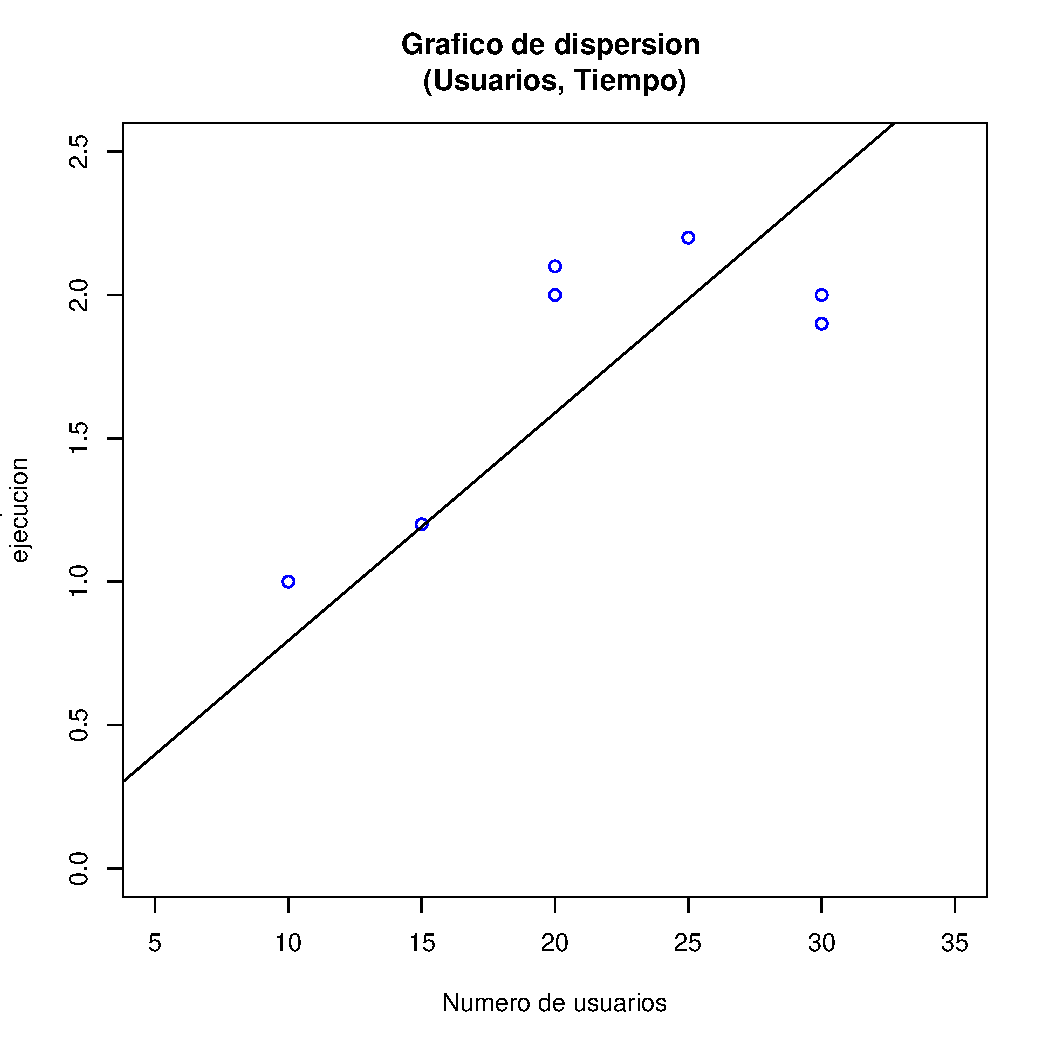
\includegraphics[width=\maxwidth]{figure/unnamed-chunk-12-1} 
\begin{kframe}\begin{alltt}
\hlcom{# Observaci\textbackslash{}'on: en la funci\textbackslash{}'on boxplot(), s\textbackslash{}'i plot es FALSE se produce un }
\hlcom{# resumen de los valores (los cinco n?meros).}

\hlcom{# Una variante del boxplot, es el notched boxplot de McGill, Larsen y Tukey, }
\hlcom{# el cual adiciona intervalos de confianza para la mediana, representados con }
\hlcom{# un par de cu\textbackslash{}~nas a los lados de la caja:}
\hlkwd{windows}\hlstd{()}
\hlkwd{boxplot}\hlstd{(X,} \hlkwc{main}\hlstd{=}\hlstr{"Grafico de caja"}\hlstd{,} \hlkwc{xlab}\hlstd{=}\hlstr{"X = Notas"}\hlstd{,} \hlkwc{notch}\hlstd{=}\hlnum{TRUE}\hlstd{,}
\hlkwc{data}\hlstd{=}\hlkwd{parent.frame}\hlstd{(),} \hlkwc{plot}\hlstd{=}\hlnum{TRUE}\hlstd{,} \hlkwc{border}\hlstd{=}\hlstr{"red"}\hlstd{,} \hlkwc{col}\hlstd{=}\hlstr{"yellow"}\hlstd{,}\hlkwc{horizontal}\hlstd{=}\hlnum{TRUE}\hlstd{)}

\hlcom{# Varios gr\textbackslash{}'aficos en una misma ventana}
\hlkwd{par}\hlstd{(}\hlkwc{mfrow}\hlstd{=}\hlkwd{c}\hlstd{(}\hlnum{1}\hlstd{,}\hlnum{2}\hlstd{))} \hlcom{# Divide la ventana gr\textbackslash{}'afica en dos partes (1 fila, 2 columnas)}
\hlkwd{mtext}\hlstd{(}\hlkwc{side}\hlstd{=}\hlnum{3}\hlstd{,} \hlkwc{line}\hlstd{=}\hlnum{0}\hlstd{,} \hlkwc{cex}\hlstd{=}\hlnum{2}\hlstd{,} \hlkwc{outer}\hlstd{=T,} \hlstr{"Titulo para Toda la Pagina"}\hlstd{)}
\end{alltt}
\end{kframe}
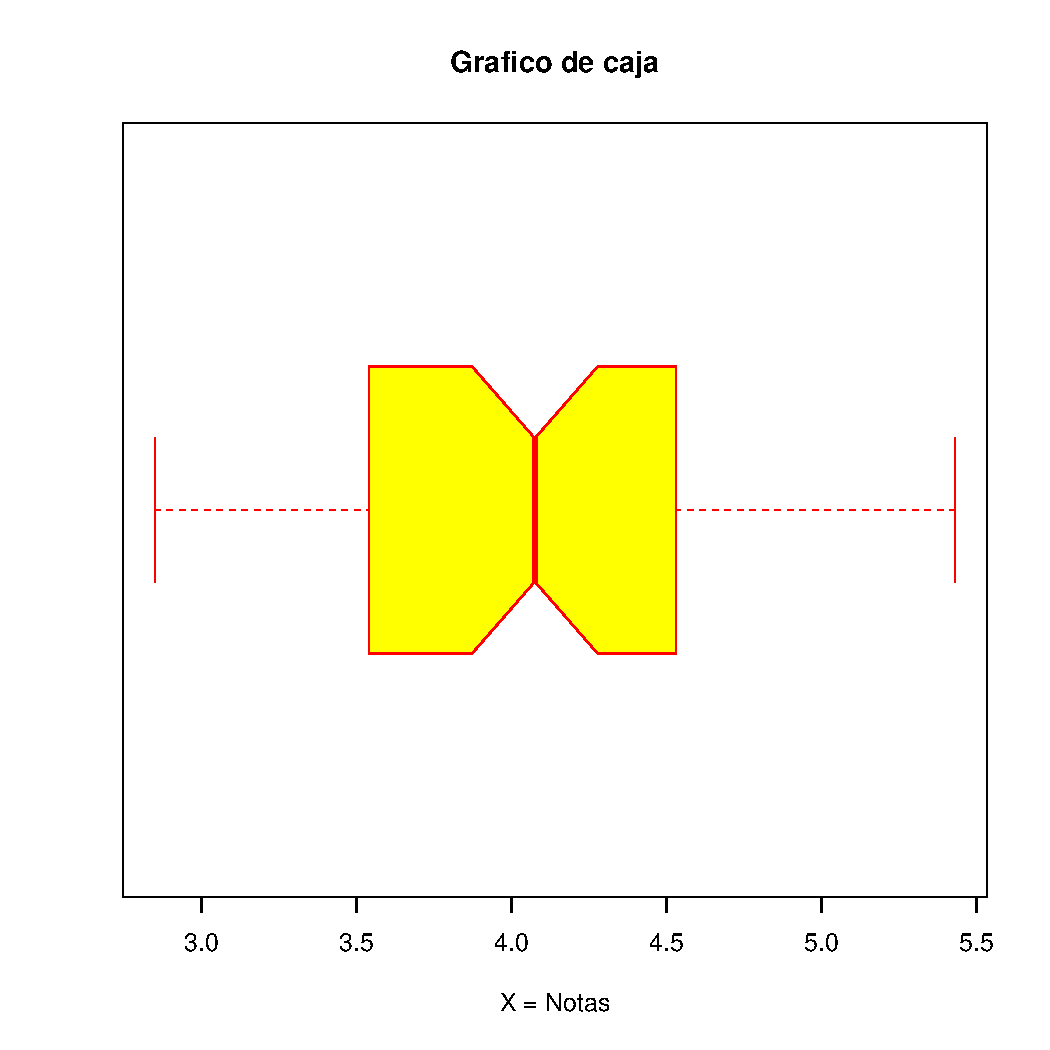
\includegraphics[width=\maxwidth]{figure/unnamed-chunk-12-2} 
\begin{kframe}\begin{alltt}
\hlkwd{hist}\hlstd{(X);}
\hlkwd{boxplot}\hlstd{(X)}
\end{alltt}
\end{kframe}
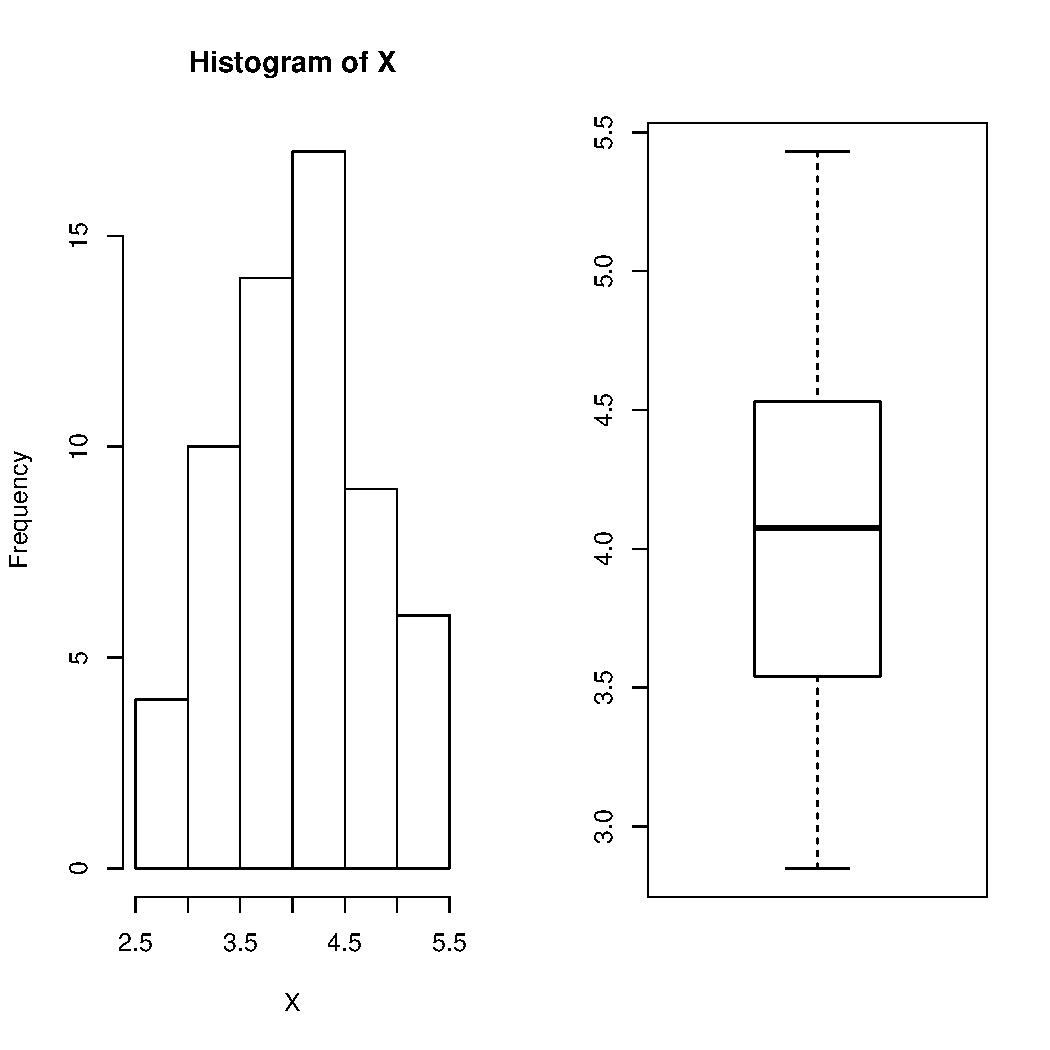
\includegraphics[width=\maxwidth]{figure/unnamed-chunk-12-3} 

\end{knitrout}


\end{document}
